\section{Conclusion}
\label{sec:conclusion}

Scaling laws promised experiments would stay cheap; however, this promise has gone unfulfilled. Today, many believe regularity only emerges at large scales, and conclusions drawn at small scales will not transfer.
%
This misconception stems from a simple, unappreciated fact: small models are much more sensitive to their hyperparameters. While scaling laws extend to very small sizes, they only emerge on the fully tuned frontier. Reaching it requires an extensive search that researchers rarely conduct. Scaling laws predict pretraining loss, and better loss does not always mean better capability; however, loss also fully captures capability---as long as the data is held fixed. Therefore, a researcher who seeks not to predict capabilities but only to improve a model can rely on loss since a model with a better law buys every loss, and thus any capability, at lower cost.

These insights suggest a new methodology of small-scale experiments, one that exploits the strong assumptions we expect to hold true while checking when they do not. Working at small scales makes this rigor affordable: we can train hundreds of models then use statistical tools, like the noisy quadratic limit, to test our assumptions. Small-scale experiments save compute, but more than that they make our conclusions more robust.

% Limitation
\textbf{Nevertheless, small-scale experiments have several limitations.} While scaling laws exist at small scales, their extrapolation hits statistical challenges. The small scale is informative, but requires judgment. Looking at the bigger picture, is the model hard to tune? Is it getting easier? How does scaling compare where we trust the law most? Instead of a single test, we should explore each of these questions using different diagnostics.
%
Perhaps the most important limitation of all, though, is the restriction to model-centric research. Changing the data breaks the perplexity--capability correspondence which pretraining loss requires to proxy for downstream tasks. With neither pretraining loss as a proxy nor reliable downstream scaling laws, small-scale experiments have limited ability to predict large-scale outcomes. Hopefully future work will unlock small-scale experiments for data-centric research; still, with care we can use small-scale experiments for model-centric research today.

% Appendix
\begin{wrapfigure}{r}{0.44\textwidth}
    \centering
    \vspace{-0.9\baselineskip}
    \definecolor{plumdark}{HTML}{4A2472}
    \definecolor{plummed}{HTML}{7B5EA7}
    \definecolor{plumlight}{HTML}{C4A0C8}
    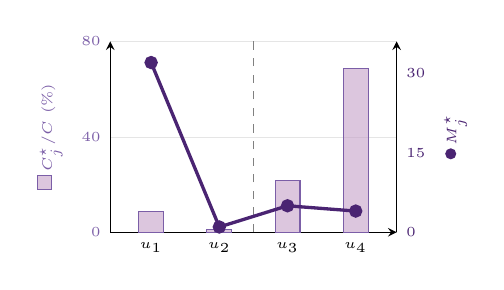
\begin{tikzpicture}
    \begin{axis}[
        name=cax,
        clip=false, scale only axis, width=0.30\textwidth, height=0.20\textwidth,
        xmin=0.4, xmax=4.6, ymin=0, ymax=80,
        axis y line=left, axis x line=bottom,
        xtick={1,2,3,4}, xticklabels={$u_1$,$u_2$,$u_3$,$u_4$},
        ytick={0,40,80}, tick label style={font=\tiny},
        ylabel={\tikz{\draw[draw=plummed, fill=plumlight, fill opacity=0.6] (0,0) rectangle (5pt,5pt);}\,$C_j^\star/C$ (\%)},
        ylabel style={font=\tiny, text=plummed},
        y tick label style={text=plummed},
        major tick length=0pt,
        ymajorgrids=true, major grid style={draw=gray!20, very thin},
    ]
      \addplot[ybar, bar width=9pt, draw=plummed, fill=plumlight, fill opacity=0.6]
          coordinates {(1,8.6) (2,1.1) (3,21.6) (4,68.7)};
      \draw[gray, dashed, thin] (axis cs:2.5,0) -- (axis cs:2.5,80);
    \end{axis}
    \begin{axis}[
        at={(cax.south west)}, anchor=south west,
        clip=false, scale only axis, width=0.30\textwidth, height=0.20\textwidth,
        xmin=0.4, xmax=4.6, ymin=0, ymax=36,
        axis y line=right, axis x line=none, xtick=\empty,
        ytick={0,15,30}, tick label style={font=\tiny},
        ylabel={\tikz{\node[circle, fill=plumdark, inner sep=0pt, minimum size=4pt]{};}\,$M_j^\star$},
        ylabel style={font=\tiny, text=plumdark},
        y tick label style={text=plumdark},
        major tick length=0pt,
    ]
      \addplot[plumdark, very thick, mark=*, mark size=1.8pt]
          coordinates {(1,32) (2,1) (3,5) (4,4)};
    \end{axis}
    \end{tikzpicture}
    \caption{
        \textbf{Getting the best scaling law fit requires different number of hyperparameter runs per scale.} The plot illustrates a typical solution, to optimizing the error at a scale $u_\star$  for a given compute budget. Because runs are cheap at $u_1$, we can run many runs while spending very little of the overall compute. The opposite is the case for the larger scale $u_4$. Another factor is the proximity to the center of the scales (dotted line). The closer a point is to the center the less influence it is going to have on the scaling law estimate, hence we are willing to make a larger mistake (see $u_2$). For the full derivation of this picture see \Cref{sec:compute-optimal-tuning}.
    }
    \label{fig:conclusion-compute-allocation}
    \vspace{-0.93\baselineskip}
\end{wrapfigure}

\textbf{Knowing what we know now, what would we change about how we design the experiments that estimate scaling laws?} Appendix~\ref{app:additional-theoretical-results} works through this question in full; here we sketch the reasoning.

First, the goal is not necessarily the most accurate scaling law, but the smallest error in the loss estimate $\hat{y}(u_\star)$ at the scale $u_\star$ we extrapolate to. And as we have shown, the two are not necessarily the same (see \Cref{fig:comparing-best-practices} for empirical and \Cref{sec:scaling-law-error-propagation} for theoretical evidence). 
A scaling law fit is similar to a linear regression in log-log space; in the linear case, we can propagate any error $\epsilon_j$ made at a small scale $u_j$ to its effect on the extrapolated prediction $\hat{y}(u_\star)$. We find that not all errors are equal, some will have a more severe effect on the prediction than others (see \Cref{fig:leverage}).
%
We then tie the error at each scale to the tuning effort spent there. With $M_j$ random-search runs at scale $u_j$, the expected error shrinks as $\epsilon_j \sim M_j^{-2/\gamma_j}$, where $\gamma_j$ is the effective number of hyperparameters at that scale (\Cref{app:background:how-close-does-random-search-get}). 

Combining both insights turns experiment design into a constrained optimization problem: given a fixed compute budget, we determine the number of runs at each scale to minimize the expected error at the target scale $u_\star$ (\Cref{sec:compute-optimal-tuning}). 
We can solve this problem in closed form. An illustration of what a solution will typically look like is in \Cref{fig:conclusion-compute-allocation}. 
 We develop this argument in full in Appendix~\ref{app:additional-theoretical-results} and distill it into a manual for designing small-scale experiments requiring the practitioner to only know their compute budget and the compute it takes to run a model at any given scale. However, executing this protocol we leave for future work.
